\documentclass[conference]{IEEEtran}
\IEEEoverridecommandlockouts
% The preceding line is only needed to identify funding in the first footnote. If that is unneeded, please comment it out.
\usepackage{cite}
\usepackage{amsmath,amssymb,amsfonts}
\usepackage{algorithmic}
\usepackage{graphicx}
\usepackage{textcomp}
\usepackage{xcolor}
\def\BibTeX{{\rm B\kern-.05em{\sc i\kern-.025em b}\kern-.08em
    T\kern-.1667em\lower.7ex\hbox{E}\kern-.125emX}}

\usepackage{biblatex} %enable for bibtex%
%mmm
\usepackage[english]{babel}
\usepackage{minted}
\usepackage{fancyvrb}
\usepackage{listings}
%for code commands in latex


%\usepackage[dvipsnames]{xcolor}
%mmm



\bibliography{template.bib}
\usepackage{comment}
 
\begin{document}

\title{Video Streaming Mixer Library*\\
{\footnotesize \textsuperscript{*}Note: Sub-titles are not captured in Xplore and
should not be used}
\thanks{Identify applicable funding agency here. If none, delete this.}
}

\author{\IEEEauthorblockN{1\textsuperscript{st} Yuni Amaloa Quintero Villalobos}
\IEEEauthorblockA{\textit{TU Berlin} \\
\textit{Fraunhofer-FOKUS-Institut  }\\
Berlin, Germany \\
Quintero.villalobos@campus.tu-berlin.de}
\and
\IEEEauthorblockN{2\textsuperscript{nd} Mohamed Mesto}
\IEEEauthorblockA{\textit{TU Berlin} \\
\textit{Fraunhofer-FOKUS-Institut  }\\
Berlin, Germany \\
m.mesto@campus.tu-berlin.de }
\and
\IEEEauthorblockN{3\textsuperscript{rd} Poonam Kumari Roy}
\IEEEauthorblockA{\textit{TU Berlin} \\
\textit{Fraunhofer-FOKUS-Institut  }\\
Berlin, Germany \\
Poonam.k.roy@campus.tu-berlin.de}

}

\maketitle

    \begin{abstract}
    Adaptive Bitrate Streaming is now the standard for the biggest streaming and video player platforms online. Data is now shared over the internet dynamically, adjusting the video resolution to the user's internet capabilities to provide a better experience. In this work, we present a proof of concept to implement two strategies that join multiple video streams into a single one only if they have matching resolutions. The motivation for this research comes from the necessity to improve the user experience and to test a new way to consume media content online. To do so, we develop a library dependency with two strategies to find matching resolutions, one that only matches the resolution of the first stream in the list, and the second, the intersection of all resolutions. Our library is implemented as a Node JS package for external applications to import. Results show the Master Manifest playlist being written with all streams content concatenated in a single one. Moreover, no playback errors were presented when the video player switches between streams as long as they have the same format regarding audio tracks. 




\begin{IEEEkeywords}
video streaming, HLS, adaptive bitrate streaming, media playlist, video segments, HLS Parser, mixer library

\end{IEEEkeywords}
    \end{abstract}

  
     
   
    \tableofcontents
    %\newpage
    \listoffigures
    \listoftables
    %\lstlistoflistings
    
    
    \section{\textbf{Introduction}}\label{sec:Introduction}
Adaptive streaming video standards are the norm for anything that is video and is streamed over the internet nowadays
For streaming adaptive video there are two main standards, MPEG-DASH and Apple‘s HLS – both similar in how they work
Instead of a single video file being transferred to clients, adaptive streaming works by splitting video into smaller segments, each segment being its own file. These video segment files are referenced by playlist files that specify time, duration and order of segments
By providing playlists and video segments playback becomes much more flexible and robust as it provides a number of benefits
Splitting of video and audio tracks, to e.g. provide multiple different audio tracks with different languages
Provide multiple video tracks with different resolution and bitrate to accomodate (temporary) bandwith bottlenecks during transfer
Being able to seamlessly switch between tracks to e.g. 720p, 1080p or 4K video resolution

\begin{figure}

\centering
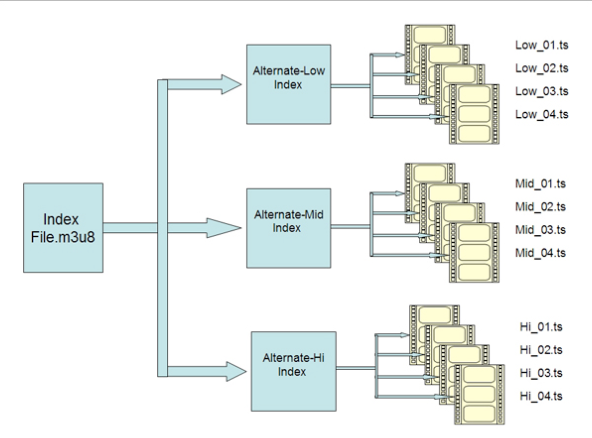
\includegraphics[scale=0.40]{figures/ProblemStatement.png}
\caption{Problem Statement \cite{rancy2016imt}}
\label{fig:IMT_2020_Use-cases}
\end{figure}


\subsection{Problem Statement
}\label{Problem Statement
}

We are in the Streaming Era

Content is transmitted without downloading

ABS dynamically changes the video source to avoid buffering

HLS splits a video file into little segments 

Not all streams share the same representations

We need an algorithm that identifies matching representation from variant video streams in order to output a single playlist












    \section{\textbf{Related Work }}\label{sec:relatedwork}

In order to create e.g. playlists consisting of multiple existing different video streams it is needed to make sure that the different video stream sources are all compatible in regards to video resolution and bitrate and can be combined into a single video stream.
Your tasks:
Parse input HLS manifests into fitting object representation
Design and implement an algorithm that identifies matching representations based on e.g. resolution, bitrate etc. 
Output must be a HLS manifest including all compatible inputs that matched
Implement as a library component that can be used in other applications as a dependency
Implement at least two separate strategies/algorithms for matching
Given an array of manifest inputs, all representations/tracks from the first manifest input need to be in the output manifest and only include the other manifest inputs if matching presentations are found
The output manifest must contain only the intersection of all representations, if nothing matches the output could be empty
Print warning messages on console for non-matching representations, print error messages to console in case nothing matched, etc

\subsection{HLS}\label{Start work}
\subsubsection{Second Stage}



Example for a Table 

 
    \section{\textbf{Our Approach}}\label{sec:main}
 \subsection{ Possible Solutions - Video Streaming Mixer Library
}


Parse HLS manifest into object representations
Implement algorithm to identify matching video streams

 \begin{itemize}

     \item Strategy 1: set Filter against first element’s attributes
     \item  Strategy 2: set intersection for matching attributes

 \end{itemize}
 The output should be a master HLS manifest of a playlist including all matching video streams

 
\begin{figure}

\centering
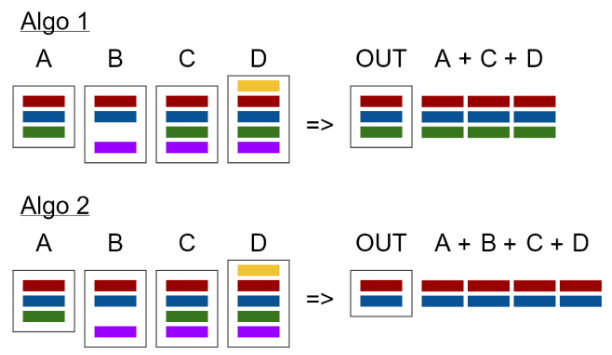
\includegraphics[scale=0.50]{figures/PossibleSolutions.png}
\caption{Possible Solutions }
\label{fig:IMT_2020_Use-cases}
\end{figure}


 
 For strategy 1, we have three variant playlists and the output also contains only three playlists. But these playlists are now longer, because they concatenate the matching playlists into a single red, a single blue and a single green playlists with all the segments from inputs A, B, C and D. While playlists purple and yellow use e.g. a different resolution and are not present in the first input A and thus are not used. 
For strategy 2, we see that only the intersection of variant playlists from all inputs is used. Two variants with the same resolution have been identified across all inputs, red and blue, so only two variant playlists should be in the output manifest. Each one will include all concatenated segments from all inputs matching the respective representation.
Finally, handling the playlists that have been identified as belonging to the same representation (resolution, bitrate). Realize that the output manifest, that needs to be written, can never have more media playlists than any of the input sources by itself. Do not add more media playlists to the master manifest. Instead, given the found media playlists using the same representation, concatenate these into a single media playlist and only that new playlist should be part of the master manifest output.




\begin{figure}

\centering
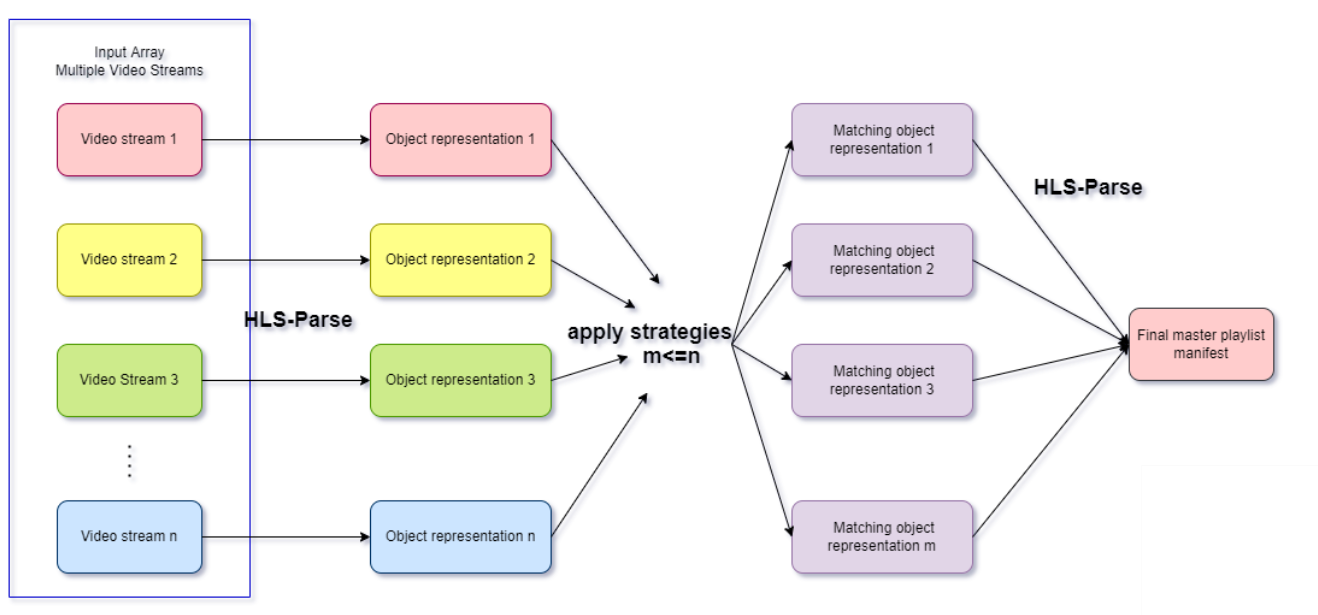
\includegraphics[scale=0.32]{figures/PossibleSolutions2.png}
\caption{Possible Solutions 2 }
\label{fig:IMT_2020_Use-cases}
\end{figure}





************************
here only to be familiar with the latex Symbols 

{\BibTeX} does not work by magic. It doesn't get the bibliographic
data from thin air but from .bib files. If you use {\BibTeX} to produce a
bibliography you must send the .bib files. 

{\LaTeX} can't read your mind. If you assign the same label to a
subsubsection and a table, you might find that Table I has been cross
referenced as Table IV-B3. 

{\LaTeX} does not have precognitive abilities. If you put a
\verb|\label| command before the command that updates the counter it's
supposed to be using, the label will pick up the last counter to be
cross referenced instead. In particular, a \verb|\label| command
should not go before the caption of a figure or a table.

Do not use \verb|\nonumber| inside the \verb|{array}| environment. It
will not stop equation numbers inside \verb|{array}| (there won't be
any anyway) and it might stop a wanted equation number in the
surrounding equation.
    \section{\textbf{Evaluation/Discussion}}\label{sec:Evaluation} 


Number equations consecutively. To make your 
equations more compact, you may use the solidus (~/~), the exp function, or 
appropriate exponents. Italicize Roman symbols for quantities and variables, 
but not Greek symbols. Use a long dash rather than a hyphen for a minus 
sign. Punctuate equations with commas or periods when they are part of a 
sentence, as in:
\begin{equation}
a+b=\gamma\label{eq}
\end{equation}

Be sure that the 
symbols in your equation have been defined before or immediately following 
the equation. Use ``\eqref{eq}'', not ``Eq.~\eqref{eq}'' or ``equation \eqref{eq}'', except at 
the beginning of a sentence: ``Equation \eqref{eq} is . . .''

\subsection{Units}
\begin{itemize}
\item Use either SI (MKS) or CGS as primary units. (SI units are encouraged.) English units may be used as secondary units (in parentheses). An exception would be the use of English units as identifiers in trade, such as ``3.5-inch disk drive''.
\item Avoid combining SI and CGS units, such as current in amperes and magnetic field in oersteds. This often leads to confusion because equations do not balance dimensionally. If you must use mixed units, clearly state the units for each quantity that you use in an equation.
\item Do not mix complete spellings and abbreviations of units: ``Wb/m\textsuperscript{2}'' or ``webers per square meter'', not ``webers/m\textsuperscript{2}''. Spell out units when they appear in text: ``. . . a few henries'', not ``. . . a few H''.
\item Use a zero before decimal points: ``0.25'', not ``.25''. Use ``cm\textsuperscript{3}'', not ``cc''.)
\end{itemize}



Be sure that the 
symbols in your equation have been defined before or immediately following 
the equation. Use ``\eqref{eq}'', not ``Eq.~\eqref{eq}'' or ``equation \eqref{eq}'', except at 
the beginning of a sentence: ``Equation \eqref{eq} is . . .''
    \section{\textbf{Conclusions}}\label{sec:conclusions}








    \input{src/00_acknowledgements}
    

    
    
    
   
    
    %\bibliographystyle{IEEEtran} % enable for bibtex
    % enable for bibtex
    \printbibliography% enable for biber style
    % to show unreferenced publications ------------------------------------- */
    %\bibliographystyle{unsrt}
    %\cite{dummy}
    %\nocite{*}
    %------------------------------------------------------------------------ */

    % /* -------------------------------------------------------------------- */




\end{document}
